    \documentclass[dvipsnames]{beamer}
    \usetheme{Madrid}
    \usefonttheme{professionalfonts}
    \usepackage{
        amsmath,
        amssymb,
        fouriernc, % fourier font w/ new century book
        fancyhdr, % page styling
        lastpage, % footer fanciness
        hyperref, % various links
        setspace, % line spacing
        amsthm, % newtheorem and proof environment
        mathtools, % \Aboxed for boxing inside aligns, among others
        float, % Allow [H] figure env alignment
        enumerate, % Allow custom enumerate numbering
        graphicx, % allow includegraphics with more filetypes
        wasysym, % \smiley!
        upgreek, % \upmu for \mum macro
        listings, % writing TrueType fonts and including code prettily
        tikz, % drawing things
        booktabs, % \bottomrule instead of hline apparently
        cancel % can cancel things out!
    }
    \usepackage[
        labelfont=bf, % caption names are labeled in bold
        font=scriptsize % smaller font for captions
    ]{caption}
    \usepackage[font=scriptsize]{subcaption} % subfigures

    \newcommand*{\scinot}[2]{#1\times10^{#2}}
    \newcommand*{\dotp}[2]{\left<#1\,\middle|\,#2\right>}
    \newcommand*{\rd}[2]{\frac{\mathrm{d}#1}{\mathrm{d}#2}}
    \newcommand*{\pd}[2]{\frac{\partial#1}{\partial#2}}
    \newcommand*{\rtd}[2]{\frac{\mathrm{d}^2#1}{\mathrm{d}#2^2}}
    \newcommand*{\ptd}[2]{\frac{\partial^2 #1}{\partial#2^2}}
    \newcommand*{\md}[2]{\frac{\mathrm{D}#1}{\mathrm{D}#2}}
    \newcommand*{\pvec}[1]{\vec{#1}^{\,\prime}}
    \newcommand*{\svec}[1]{\vec{#1}\;\!}
    \newcommand*{\bm}[1]{\boldsymbol{\mathbf{#1}}}
    \newcommand*{\ang}[0]{\;\text{\AA}}
    \newcommand*{\mum}[0]{\;\upmu \mathrm{m}}
    \newcommand*{\at}[1]{\left.#1\right|}

    \let\Re\undefined
    \let\Im\undefined
    \DeclareMathOperator{\Res}{Res}
    \DeclareMathOperator{\Re}{Re}
    \DeclareMathOperator{\Im}{Im}
    \DeclareMathOperator{\Log}{Log}
    \DeclareMathOperator{\Arg}{Arg}
    \DeclareMathOperator{\Tr}{Tr}
    \DeclareMathOperator{\E}{E}
    \DeclareMathOperator{\Var}{Var}
    \DeclareMathOperator*{\argmin}{argmin}
    \DeclareMathOperator*{\argmax}{argmax}
    \DeclareMathOperator{\sgn}{sgn}
    \DeclareMathOperator{\diag}{diag\;}

    \DeclarePairedDelimiter\bra{\langle}{\rvert}
    \DeclarePairedDelimiter\ket{\lvert}{\rangle}
    \DeclarePairedDelimiter\abs{\lvert}{\rvert}
    \DeclarePairedDelimiter\ev{\langle}{\rangle}
    \DeclarePairedDelimiter\p{\lparen}{\rparen}
    \DeclarePairedDelimiter\s{\lbrack}{\rbrack}
    \DeclarePairedDelimiter\z{\lbrace}{\rbrace}

    % \everymath{\displaystyle} % biggify limits of inline sums and integrals
    \tikzstyle{circ} % usage: \node[circ, placement] (label) {text};
        = [draw, circle, fill=white, node distance=3cm, minimum height=2em]
    \definecolor{commentgreen}{rgb}{0,0.6,0}
    \lstset{
        basicstyle=\ttfamily\footnotesize,
        frame=single,
        numbers=left,
        showstringspaces=false,
        keywordstyle=\color{blue},
        stringstyle=\color{purple},
        commentstyle=\color{commentgreen},
        morecomment=[l][\color{magenta}]{\#}
    }

\begin{document}

\title{Cassini State Separatrix Hopping}
\subtitle{Group Meeting Presentation}
\author{Yubo Su}
\date{Apr 19, 2019}

\maketitle

\begin{frame}
    \frametitle{Cassini States}
    \framesubtitle{Introduction}

    \begin{columns}
        \begin{column}{0.45\textwidth}
            \begin{figure}[t]
                \centering
                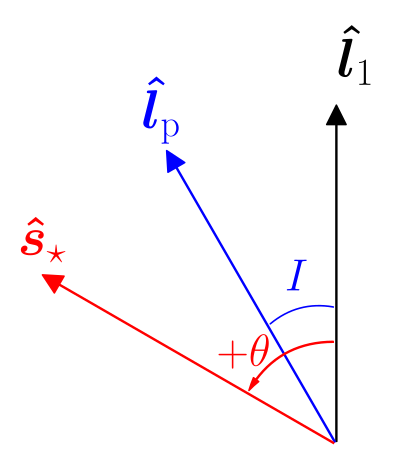
\includegraphics[width=0.7\textwidth]{plots/cassini.png}
            \end{figure}
        \end{column}
        \begin{column}{0.45\textwidth}
            \begin{itemize}
                \item In corotating ($\hat{l}_p$ fixed) frame,
                    \begin{equation*}
                        \rd{\hat{s}}{t}
                            = \p*{\hat{s} \cdot \hat{l}_1}
                                \p*{\hat{s} \times \hat{l}_1} - \eta
                                    \p*{\hat{s} \times \hat{l}_p}.
                    \end{equation*}
                \begin{itemize}
                    \item $\eta = \frac{\abs*{g}}{\alpha}$: $g$ is $\hat{l}_1$
                        precession around total angular momentum axis, $\alpha$ spin
                        precession.
                \end{itemize}
                \item Hamiltonian
                    \begin{equation*}
                        \mathcal{H} = \frac{\p*{\hat{s} \times \hat{l}_1}^2}{2}
                            - \eta\p*{\hat{s} \cdot \hat{l}_p}.
                    \end{equation*}
            \end{itemize}
        \end{column}
    \end{columns}
\end{frame}

\begin{frame}
    \frametitle{Cassini States}
    \framesubtitle{Separatrix}

    \begin{figure}[t]
        \centering
        \includegraphics[width=0.7\textwidth]{../initial/plots/1contours.png}
        \caption{Black line corresponds to \emph{separatrix}. Equipotential
        surface joining two saddle points, \emph{flows cannot cross}. Area can
        be numerically estimated.}
    \end{figure}
\end{frame}

\begin{frame}
    \frametitle{Cassini States}
    \framesubtitle{Separatrix}

    \begin{columns}
        \begin{column}{0.45\textwidth}
            \begin{figure}[t]
                \centering
                \includegraphics[width=\textwidth]{../initial/plots/4_01contour.png}
                \caption{Red, purple Cassini states are stable,
                \emph{attracting} with dissipation.}
            \end{figure}
        \end{column}
        \begin{column}{0.45\textwidth}
            \begin{itemize}
                \item Zoom in on $\eta = 0.1$ case (left).

                \item \textbf{If weak dissipation \& random IC,
                    what is fate of system?}

                \item \emph{Hypothesis:}
                    \begin{description}
                        \item[Outside] Alignment (77.1\%)
                        \item[Inside] High obliquity (22.9\%)
                    \end{description}
            \end{itemize}
        \end{column}
    \end{columns}
\end{frame}

\begin{frame}
    \frametitle{Cassini States}
    \framesubtitle{Simulations}

    Introduce tidal force $\p*{\rd{\hat{s}}{t}}_{tide} = \epsilon \hat{s} \times
    \p*{\hat{l}_1 \times \hat{s}} = -\epsilon \sin\theta\hat{\theta}$. Fate?

    \begin{figure}[t]
        \centering
        \includegraphics[width=0.65\textwidth]{../initial/plots/3stats3_5_0_1.png}
        \caption{In other sims $\epsilon \to 0$, $P_{hop} \to 0.08$, \emph{nonzero}!}
    \end{figure}
\end{frame}

\begin{frame}
    \frametitle{Cassini States}
    \framesubtitle{Separatrix Hopping}

    \begin{columns}
        \begin{column}{0.47\textwidth}
            \begin{itemize}
                \item \emph{Revised hypothesis}: \textbf{74\%} align,
                    \textbf{26\%} high obliquity,
                    \begin{description}
                        \item[Above] Goes to alignment (38.55\%)
                        \item[Inside] High obliquity (22.9\%)
                        \item[Below] High-obliquity 8\% (3.1\%),
                            rest align (35.55).
                    \end{description}

                \item Data: \textbf{73.4\%} align, \textbf{25.9\%}
                    high obliquity!
            \end{itemize}
        \end{column}
        \begin{column}{0.47\textwidth}
            \begin{figure}[t]
                \centering
                \includegraphics[width=\textwidth]{../initial/plots/4singles.png}
                \caption{Trajectories at moment of crossing $\theta_4$,
                converging to two attracting CSs.}
            \end{figure}
        \end{column}
    \end{columns}
\end{frame}

\begin{frame}
    \frametitle{Separatrix Hopping}
    \framesubtitle{Heteroclinic Orbits}

    \begin{columns}
        \begin{column}{0.47\textwidth}
            \begin{figure}[t]
                \centering
                \includegraphics[width=\textwidth]{../initial/plots/3stats2_0_0_1.png}
            \end{figure}
        \end{column}
        \begin{column}{0.47\textwidth}
            \begin{figure}[t]
                \centering
                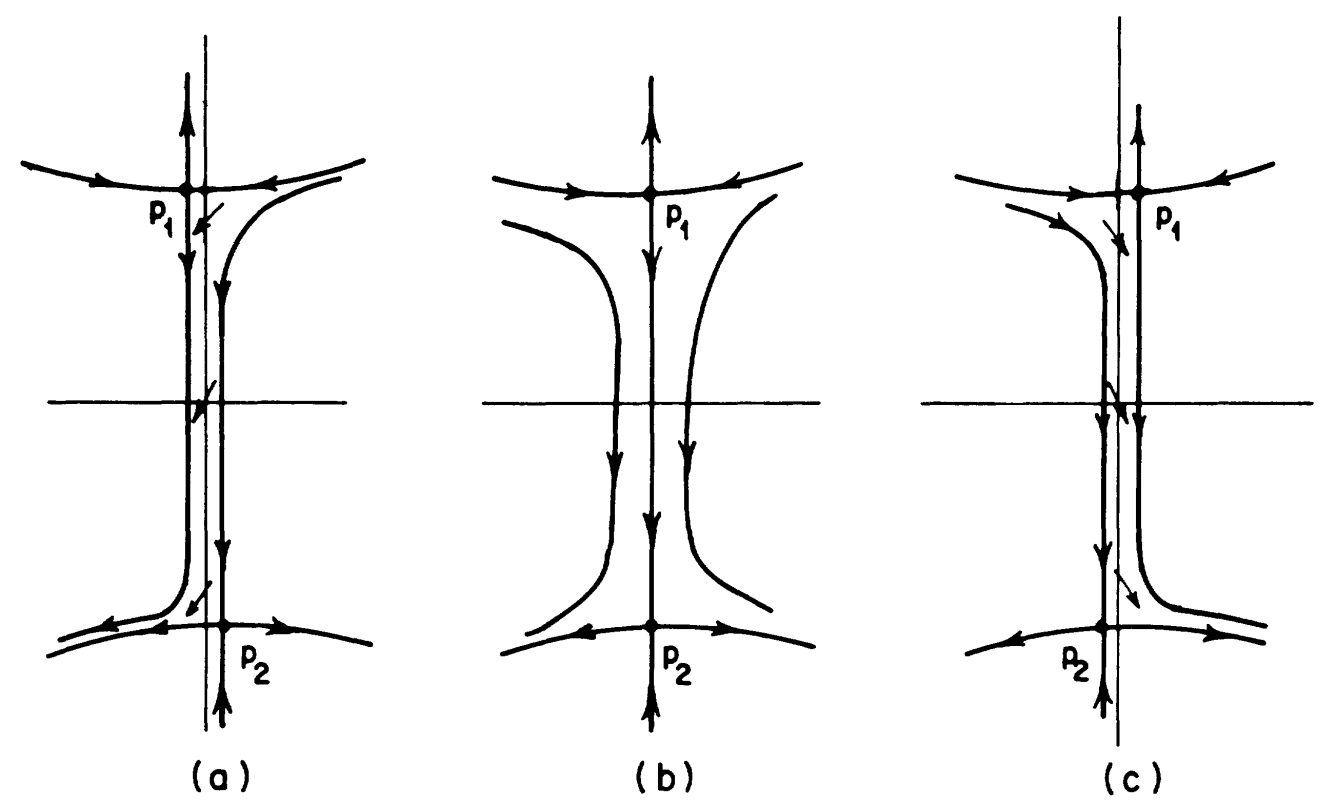
\includegraphics[width=\textwidth]{plots/heteroclinic.png}
                \caption{Heteroclinic orbit (\emph{separatrix}) under perturbation.}
            \end{figure}
        \end{column}
    \end{columns}
\end{frame}

\begin{frame}
    \frametitle{Separatrix Hopping}
    \framesubtitle{Hypothesis}

    \begin{itemize}
        \item Modified Cassini state under tides, $\delta \phi_4 =
            +\frac{\epsilon}{\eta \sin I}$.

        \item Opens gap $\propto \epsilon$, but alignment strength also $\propto
            \epsilon$ (draw).

        \item Thus, hopping probability $\propto \mathcal{O}(\epsilon^2)$.
    \end{itemize}
    \begin{figure}[t]
        \centering
        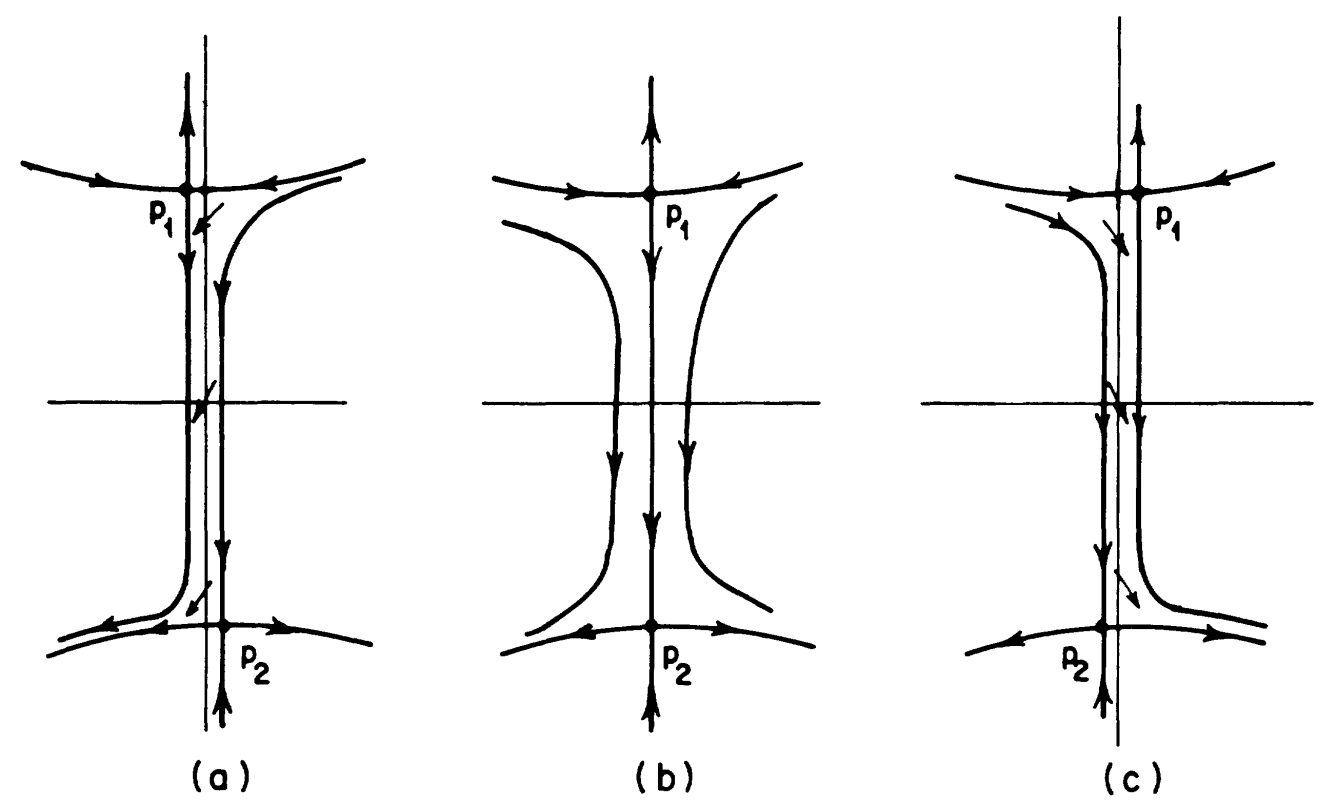
\includegraphics[width=0.6\textwidth]{plots/heteroclinic.png}
        \caption{Heteroclinic orbit (\emph{separatrix}) under perturbation.}
    \end{figure}
\end{frame}

\begin{frame}
    \frametitle{Separatrix Hopping}
    \framesubtitle{Varying $\eta$}

    \begin{itemize}
        \item Tried varying $\eta$, fixed $\epsilon$. Maybe $P_{hop} \propto
            \eta A$?:
            \begin{table}[t]
                \centering
                \begin{tabular}{c | c c c c}
                    $\eta$ & $0.025$ & $0.05$ & $0.1$ & $0.2$\\\midrule
                    $P_{hop}$ & $0.01$ & $0.028$ & $0.08$ & $0.25$\\\midrule
                    $A$ & $0.115$ & $0.163$ & $0.229$ & $0.320$
                \end{tabular}
            \end{table}
    \end{itemize}
    \begin{figure}[b]
        \centering
        \includegraphics[width=0.5\textwidth]{../initial/plots/3stats3_5_0_2.png}
    \end{figure}
\end{frame}

\end{document}

